% 本试卷单独编译时不显示页眉，保留页码。
\pagestyle{plain}

\begin{center}
  {\Large\bfseries 人大附中2027届高三暑假自主复习检测练习\par}
  \vspace{0.5em}
  {\Large\bfseries 数\quad 学}
\end{center}

\noindent 说明：本试卷共21道题，共150分；考试时间120分钟；请在答题纸上填写个人信息，并将条形码贴在答题纸的相应位置上。

\subsection*{第一部分（选择题\quad 共40分）}

\noindent\textbf{一、选择题}（本大题共10小题，每小题4分，共40分。在每小题给出的四个选项中，只有一项是符合题目要求的。）

\noindent 1. 已知集合$A=\{y\in\mathbb{N}\mid y^2+y-6\leqslant0\}$，$B=\{t\mid |t|>1\}$，则$A\cap B$为（\quad）
\begin{multicols}{4}
\begin{enumerate}[label=\Alph*.,leftmargin=*]
  \item $\varnothing$
  \item $2$
  \item $\{2,3\}$
  \item $\{2\}$
\end{enumerate}
\end{multicols}

\noindent 2. 已知$z=3-4\mathrm{i}$，则在复平面上，复数$z$所对应的点在（\quad）
\begin{multicols}{4}
\begin{enumerate}[label=\Alph*.,leftmargin=*]
  \item 第一象限
  \item 第二象限
  \item 第三象限
  \item 第四象限
\end{enumerate}
\end{multicols}

\noindent 3. 下列函数中，是奇函数并且经过函数图像上任意两点的直线斜率均为负的是（\quad）
\begin{center}
\begin{tabular}{@{}p{0.47\textwidth}p{0.47\textwidth}@{}}
A. $f(x)=\dfrac{1}{1+x^2}$
  & B. $f(x)=\lg\!\left(-x+\sqrt{x^2+1}\right)$ \\
C. $f(x)=\dfrac{\mathrm{e}^x-\mathrm{e}^{-x}}{2}$
  & D. $f(x)=-x\cos x$
\end{tabular}
\end{center}

\noindent 4. 已知实数$a,b$满足$a>b$，则（\quad）
\begin{multicols}{4}
\begin{enumerate}[label=\Alph*.,leftmargin=*]
  \item $a^5>b^3$
  \item $\sqrt[5]{a}>\sqrt[3]{b}$
  \item $5+a>3+b$
  \item $5a>3b$
\end{enumerate}
\end{multicols}

\noindent 5. 已知直线$l:4x+3y=0$和圆$C:(x-4)^2+(y-3)^2=4$，点$P$在直线$l$上，点$Q$在圆$C$上，则$|PQ|$最小值为（\quad）
\begin{multicols}{4}
\begin{enumerate}[label=\Alph*.,leftmargin=*]
  \item $1$
  \item $3$
  \item $6$
  \item $9$
\end{enumerate}
\end{multicols}

\noindent 6. 在下列双曲线中，离心率最大的是（\quad）
\begin{center}
\begin{tabular}{@{}p{0.47\textwidth}p{0.47\textwidth}@{}}
A. $\dfrac{x^2}{4}-\dfrac{y^2}{5}=1$
  & B. $\dfrac{x^2}{5}-\dfrac{y^2}{6}=1$ \\
C. $\dfrac{y^2}{6}-\dfrac{x^2}{7}=1$
  & D. $\dfrac{y^2}{7}-\dfrac{x^2}{8}=1$
\end{tabular}
\end{center}

\noindent 7. 设函数$f(x)=a\sin\omega x+b\cos\omega x$，$(a,b\in\mathbb{R},ab\neq0,\omega>0)$，若$f(x)\geqslant f\!\left(\dfrac{\pi}{3}\right)$对任意实数$x$均成立，则下列结论中一定不成立的是（\quad）
\begin{center}
\begin{tabular}{@{}p{0.47\textwidth}p{0.47\textwidth}@{}}
A. $\forall x\in\mathbb{R}$，总有$f(x)=f(-x)$
  & B. $\forall x\in\mathbb{R}$，总有$f(x)=-f(-x)$ \\
C. $\forall x\in\mathbb{R}$，总有$f\!\left(\dfrac{2\pi}{3}+x\right)=f(-x)$
  & D. $\forall x\in\mathbb{R}$，总有$f\!\left(\dfrac{2\pi}{3}+x\right)=-f(-x)$
\end{tabular}
\end{center}

\noindent 8. 已知$\{a_n\}$是各项均为正数的无穷数列，记集合
\[
T_n=\left\{t\,\middle|\,t=\frac{a_i-a_n}{i-n},\ i=1,2,\ldots,n-1,n+1,\ldots\right\},
\]
则“数列$\{a_n\}$是等差数列”是“对于任意正整数$n$，集合$T_n$都是单元素集，且该元素为正数”的（\quad）
\begin{center}
\begin{tabular}{@{}p{0.47\textwidth}p{0.47\textwidth}@{}}
A. 充分不必要条件 & B. 必要不充分条件 \\
C. 充分必要条件   & D. 既不充分又不必要条件
\end{tabular}
\end{center}

\noindent 9. 激活函数在神经网络中的核心作用是引入非线性变换，使得神经网络可以学习和模拟复杂函数关系，从而解决线性模型无法处理的非线性问题。一个常见的激活函数为
\[
\operatorname{Tanh}(x)=\frac{\mathrm{e}^x-\mathrm{e}^{-x}}{\mathrm{e}^x+\mathrm{e}^{-x}}.
\]
如果$|\operatorname{Tanh}(x_1)-\operatorname{Tanh}(x_2)|=1$，则$|x_1-x_2|$最小值最接近的数为（\quad）

\noindent（参考数据：$\ln2=0.69$，$\ln3=1.10$，$\ln5=1.61$）
\begin{multicols}{4}
\begin{enumerate}[label=\Alph*.,leftmargin=*]
  \item $0.42$
  \item $0.55$
  \item $0.69$
  \item $1.10$
\end{enumerate}
\end{multicols}

\noindent 10. 已知向量$\vec a=(1,0)$，$|\vec b|=\sqrt3$，$\vec a\cdot\vec b=0$，若向量$\vec c$满足$|\vec c|=2$且$|\vec c-\vec b|-|\vec c-\vec a|=2$，则符合条件的向量$\vec c$的个数为（\quad）
\begin{multicols}{4}
\begin{enumerate}[label=\Alph*.,leftmargin=*]
  \item $0$
  \item $2$
  \item $4$
  \item $6$
\end{enumerate}
\end{multicols}

\subsection*{第二部分（非选择题\quad 共110分）}

\noindent\textbf{二、填空题}（本大题共5小题，每小题5分，共25分。）

\noindent 11. 抛物线$y=2x^2$的准线上一点到其焦点的最小距离为\underline{\hspace{3cm}}。

\noindent 12. 在$(x-a)^6$的展开式中，若$x^5$的系数为$12$，则$a$的值为\underline{\hspace{3cm}}。

\noindent 13. 中国古代以“三分损益法”确定十二律管的长度，从“黄钟”出发，交替进行“损一”和“益一”操作，依次生得十二律管。记“黄钟”长度为$a_1=1$，第$n$次损益后得到的律管长度为$a_{n+1}$（$n=1,2,\ldots,11$），已知损益规则为
\[
a_{n+1}=\begin{cases}
\dfrac23a_n,&n\text{为奇数},\\[4pt]
\dfrac43a_n,&n\text{为偶数},
\end{cases}
\]
则$a_1+a_3+a_5+a_7+a_9+a_{11}=$\underline{\hspace{3cm}}。

\noindent 14. 如图，五面体$ABC-DEF$满足$AD\parallel BE\parallel CF$，且三条平行线两两间距离均为$2$。若$AD=1$，$BE=2$，$CF=3$，则该五面体的体积为\underline{\hspace{3cm}}。

\begin{center}
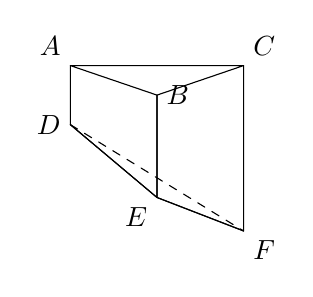
\begin{tikzpicture}[scale=0.5,line join=round,line cap=round]
  \coordinate (A) at (0,2.2);
  \coordinate (B) at (2.2,1.45);
  \coordinate (C) at (4.4,2.2);
  \coordinate (D) at (0,0.7);
  \coordinate (E) at (2.2,-1.15);
  \coordinate (F) at (4.4,-2.0);
  \draw (A)--(B)--(C)--cycle;
  \draw (A)--(D)--(E)--(B);
  \draw (B)--(E)--(F)--(C);
  \draw (C)--(F);
  \draw (D)--(E)--(F);
  \draw[dashed] (D)--(F);
  \foreach \P/\pos in {A/above left,B/right,C/above right,D/left,E/below left,F/below right}
    \node[\pos] at (\P) {$\P$};
\end{tikzpicture}
\end{center}

\noindent 15. 函数
\[
f(x)=\begin{cases}
-x^2+2ax+1,&x\leqslant-a,\\
\ln(x+a),&x>-a,
\end{cases}
\qquad a\in\mathbb{R},
\]
给出下列四个结论：

\noindent ①函数$f(x)$的值域为$\mathbb{R}$；

\noindent ②$a=0$时，存在区间$(s,t)$，使得$f(x)$在$(s,t)$上单调递减；

\noindent ③$a<0$时，$f(x)$至少有一个极值点；

\noindent ④若关于$x$的方程$[f(x)]^2=f(x)$的解集有5个元素，则$a$的取值范围为$\left(0,\dfrac{\sqrt3}{3}\right]$。

\noindent 其中正确结论的序号是\underline{\hspace{3cm}}。
\newpage
\noindent\textbf{三、解答题}（本大题共6小题，共85分。解答应写出文字说明、演算步骤或证明过程。）

\noindent 16. 已知$\triangle ABC$中，$c=6$，$a=5$，$C=2A$。

\noindent（1）求$\cos C$的值；

\noindent（2）求$\triangle ABC$的面积。
\newpage
\noindent 17. 四棱锥$B-AA_1C_1C$中，底面$AA_1C_1C$是正方形，$D$是棱$BC_1$上一个点，平面$ABC\perp$平面$AA_1C_1C$。

\begin{center}
\begin{tikzpicture}[scale=0.85,line join=round,line cap=round]
  \coordinate (A)  at (0,0);
  \coordinate (A1) at (0.2,3.0);
  \coordinate (C1) at (-1.5,1.9);
  \coordinate (C)  at (-1.7,-1.1);
  \coordinate (B)  at (3.5,-0.1);
  \coordinate (D)  at ($(C1)!0.58!(B)$);

  % 底面正方形 AA_1C_1C，被遮挡的棱用虚线表示
  \draw[dashed] (A)--(A1);
  \draw (A1)--(C1)--(C);
  \draw[dashed] (C)--(A);

  % 四棱锥的侧棱
  \draw (B)--(A1);
  \draw (B)--(C1);
  \draw (B)--(C);
  \draw[dashed] (B)--(A);

  % D 位于 BC_1 上，补出 AD 与 A_1D
  \draw[dashed] (A)--(D);
  \draw[thick] (A1)--(D);
  \fill (D) circle (1.3pt);

  \node[below left]  at (A)  {$A$};
  \node[above]       at (A1) {$A_1$};
  \node[left]        at (C1) {$C_1$};
  \node[below left]  at (C)  {$C$};
  \node[right]       at (B)  {$B$};
  \node[above right] at (D)  {$D$};
\end{tikzpicture}
\end{center}

\noindent（1）若$AD\perp BC$，求证：$A_1D\perp BC$；

\noindent（2）若$AB=AC=AA_1=2$，$D$是$BC_1$中点，再从条件①、条件②、条件③这三个条件中选择一个作为已知，使得四棱锥$B-AA_1C_1C$存在且唯一确定。求直线$A_1D$与平面$BCC_1$所成角的正弦值。

\noindent 条件①：$BD=\dfrac12BC$；

\noindent 条件②：$BC=2\sqrt2$；

\noindent 条件③：$\angle BC_1C=\angle BC_1A_1$。
\newpage
\noindent 18. 甲、乙两人进行飞碟射击比赛，共比赛10场，规定每场比赛分数最高者获胜，两人得分（单位：分）情况统计如下：

\begin{center}
\renewcommand{\arraystretch}{1.45}
\setlength{\tabcolsep}{0.75em}
\begin{tabular}{|c|*{10}{c|}}
  \hline
  场次&1&2&3&4&5&6&7&8&9&10\\ \hline
  甲&9&13&8&12&14&11&7&9&12&10\\ \hline
  乙&8&11&10&7&12&8&8&10&10&13\\ \hline
\end{tabular}
\end{center}

\noindent 用频率估计概率。

\noindent（1）从上述10场比赛中随机选择一场，在甲获胜的前提下，求分差超过3分的概率；

\noindent（2）从这10场比赛中任选3场，设$X$表示抽到的3场中甲获胜的场数，求$X$的分布列和数学期望；

\noindent（3）记一次飞碟比赛成绩满分为15分，设$n$名运动员的得分分别为$a_1,a_2,\ldots,a_n$（$a_i\in\mathbb{N},1\leqslant i\leqslant n$），$b_k$（$1\leqslant k\leqslant15$）为$n$名运动员中得分至少为$k$分的人数。记$M$为$n$名运动员的平均成绩，$N=\dfrac{b_1+b_2+\cdots+b_{15}}{n}$，直接写出$M,N$的大小关系（结论不用证明）。
\newpage
\noindent 19. 已知椭圆$E:\dfrac{x^2}{a^2}+\dfrac{y^2}{b^2}=1$（$a>b>0$）的左、右顶点分别为$A(-a,0),B(a,0)$，右焦点$F(c,0)$，$|FA|=3|FB|$，$|AB|=8$。动点$T,S$均在椭圆$E$上（不同于顶点），直线$AS$交$y$轴于点$M$，直线$BT$交$y$轴于点$N$。

\noindent（1）求椭圆$E$的方程和离心率；

\noindent（2）若点$M,N$满足$3\overrightarrow{OM}=-5\overrightarrow{ON}$，试判断直线$TS$是否经过定点。如果是，求出该定点坐标；如果不是，说明理由。

\begin{solution}
\begingroup
\setlength{\abovedisplayskip}{3pt}
\setlength{\belowdisplayskip}{3pt}
\setlength{\abovedisplayshortskip}{2pt}
\setlength{\belowdisplayshortskip}{2pt}
\noindent（1）由$|AB|=2a=8$，得$a=4$。

因为$|FA|=a+c$，$|FB|=a-c$，所以$a+c=3(a-c)$，解得$c=2$。从而
$b^2=a^2-c^2=12$。因此
\[
\boxed{\frac{x^2}{16}+\frac{y^2}{12}=1},
\qquad e=\frac ca=\boxed{\frac12}.
\]

\noindent（2）设直线$AS$的斜率为$k$，则$AS:y=k(x+4)$，所以$M(0,4k)$。
设直线$BT$的斜率为$t$，则$BT:y=t(x-4)$，所以$N(0,-4t)$。由
$3\overrightarrow{OM}=-5\overrightarrow{ON}$得$12k=20t$，即
\[
t=\frac35k. \tag{1}
\]

将直线$AS$与椭圆$E$联立。利用$A(-4,0)$是其中一个交点，得另一个交点$S$。
同理可得点$T$，两点坐标为
\[
\begin{aligned}
S&\left(\frac{4(3-4k^2)}{3+4k^2},\frac{24k}{3+4k^2}\right),\\
T&\left(\frac{4(4t^2-3)}{3+4t^2},-\frac{24t}{3+4t^2}\right).
\end{aligned}
\]

由点$S,T$的坐标写出直线$ST$的方程，整理得
\[
3(k+t)x+(4kt-3)y-12(t-k)=0.
\]
将式（1）代入，得直线$ST$的方程为
\[
8k(x+1)+(4k^2-5)y=0. \tag{2}
\]

设所有直线$ST$共同经过点$P(x_0,y_0)$。将$P$的坐标代入式（2），得
\[
4y_0k^2+8(x_0+1)k-5y_0=0.
\]
因为上式对变化的$k$恒成立，所以
\[
\begin{cases}
4y_0=0,\\
8(x_0+1)=0,\\
-5y_0=0.
\end{cases}
\]
解得
\[
x_0=-1,\qquad y_0=0.
\]
因此，直线$TS$经过定点，该定点为
\[
\boxed{(-1,0)}.
\]
\endgroup
\end{solution}
\newpage
\noindent 20. 已知函数$f(x)=x\mathrm{e}^{x-a}$。

\noindent（1）$a=-1$时，求曲线$y=f(x)$与$x$轴平行的切线方程；

\noindent（2）已知函数$g(x)=\dfrac12x^2-x$。

\noindent\quad (i) 当$a<0$时，求曲线$y=f(x)$与曲线$y=g(x)$的交点个数；

\noindent\quad (ii) 如果存在实数$t$，使得两条曲线在$x=t$处有公共点，且两条曲线在$x=t$处的导数也相同，则称这两条曲线相切。求$a$的值，使得曲线$y=f(x)$与曲线$y=g(x)$相切。
\newpage
\noindent 21. 给定正整数$n\geqslant3$，集合
\[
M=\{(x,y)\mid x\in\{1,2,\ldots,n\},\ y\in\{1,2,\ldots,n\}\},
\]
从$M$中选取不同的$m$个元素组成一个向量序列
\[
(x_1,y_1),(x_2,y_2),\ldots,(x_m,y_m),
\]
若该序列同时满足如下两条性质：

\noindent ①$(x_1,y_1)=(1,1)$，$x_m=n$；

\noindent ②$\vec a_i=(x_i,y_i)$，$\vec a_{i+1}-\vec a_i\in\{(1,0),(0,1),(0,-1)\}$，$i=1,2,3,\ldots,m-1$，

\noindent 则称该序列为$S$列。

\noindent（1）当$n=3$时，分别判断向量序列
\[
A:(1,1),(2,1),(2,2),(3,1),\qquad
B:(1,1),(1,2),(2,2),(2,1),(3,1)
\]
是否是$S$列（结论无需证明）。

\noindent（2）当$n=4$时，是否存在一个由$M$的全部元素组成的$S$列，满足$(x_m,y_m)=(n,n)$，并说明理由；

\noindent（3）若$S$列$(x_1,y_1),(x_2,y_2),\ldots,(x_m,y_m)$满足条件
\[
\{y_i\mid i=1,2,\ldots,m\}=\{1,2,\ldots,n\},
\]
求这样的$S$列的个数。
